%07chapterZusammenfasssung.tex

\chapter{Interview}


\section{Interviewleitfaden}

Die Interviewleitfragen wurden mithilfe der Website \cite{Schluesselqualifikationen} erstellt. Daraus wurden zehn Schlüsselkompetenzen ausgewählt und eine Umfrage erstellt, womit die Wichtigkeit der einzelnen Schlüsselkompetenzen im Alltag eines Junior Elektroingenieur ermittelt werden sollten. Die Fragen konnten jeweils mit \textbf{sehr wichtig}, \textbf{ziemlich wichtig} und \textbf{nicht wichtig} markiert werden. (Siehe Interviewteil im Anhang (\ref{sec:Interviews}))  

\section {Technische Hilfsmittel}

Der Fragebogen wurde mit Latex erstellt. Da uns klar war, dass für das Ausfüllen einer Umfrage oft der Aufwand das grösste Hindernis darstellt, haben wir uns für ein interaktives PDF-Design entschieden. Das bedeutet, dass alle benötigten Informationen direkt ins PDF eingetragen werden können. Damit die Teilnehmer sich nicht mit dem Absenden der Mails beschäftigen müssen, haben wir noch ein ''Submit-Button'' hinzugefügt, der das File direkt an uns weiterleitet. Diese Vorkehrungen sollten sicherstellen, dass wir möglichst viele Antworten erhalten und die Signifikanz steigt. 

%\footnote{Text}

\section{Interviewpartner Auswahl}

Die erstellten Umfragen haben wir anschliessend jeweils zwei bis drei uns bekannten Elektroingenieuren zugeschickt. Von den acht zugeschickten Formularen, haben wir fünf ausgefüllt zurückbekommen ((\ref{sec:Interviews})). 

\section{Auswertung der Interviews}

Die Auswertung der Formulare erfolgte mittels einer einfachen Excel Tabelle \ref{fig:tabkernkomp}. Um herauszufinden welche Schlüsselkompetenzen wichtig waren, wurden pro Schlüsselkompetenz Punkte verteilt. Dabei entsprach ''sehr Wichtig'' plus einem Punkt, ''ziemlich wichtig'' null Punkten und ''nicht Wichtig'' minus einem Punkt. Die Summe der Punkte ist im Bild \ref{fig:auswerkomp} dargestellt. 

\begin{figure}[ht]
	\centering
	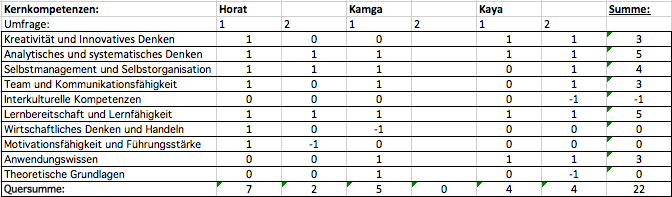
\includegraphics[width=1.2\textwidth]{images/Tabelle_Kernkompetenzen.png}
	\caption{Tabelle Kernkompetenzen}
	\label{fig:tabkernkomp}
\end{figure}

\begin{figure}[ht]
	\centering
	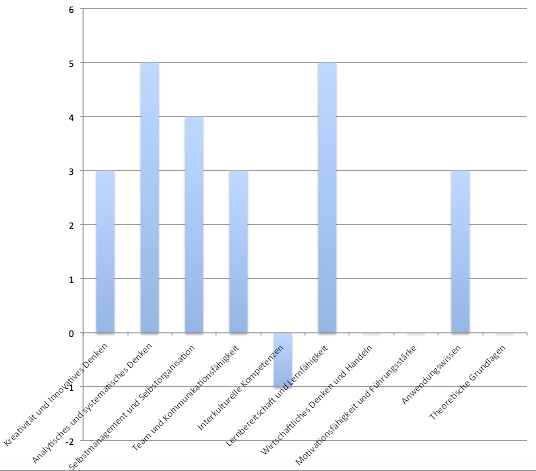
\includegraphics[width=1.1\textwidth]{images/Auswertung_kernkompetenzen.png}
	\caption{Auswertung Kernkompetenzen}
	\label{fig:auswerkomp}
\end{figure}


Interessant sind unter anderem, dass Interkulturelle Kompetenzen als die unwichtigste Kompetenz bewertet wurde. Auch schienen die Befragten die theoretischen Grundlagen als kaum relevant einzuschätzen.

